%%%%%%%%%%%%%%%%%%%%%%%%%%%%%%%%%%%%%%%%%%%%%%%%%%%%%%%%%%%%%%%%%%%%%%%%%%%%%%

\chapter{THEORETICAL BACKGROUND}\label{ch:fun}

This chapter presents the theoretical background necessary to understand the concepts in this thesis, starting with satellite operations, the definitions of Big Data, Data Warehouse, OLAP and Data Cubes.

\section{Satellite Operations}\label{ch:fun:operations}

A satellite is divided into two modules: the service module and the payload.
The service module is composed of everything necessary for the operation of the on-board equipment, such as the power supply system, the ground communication system, the on-board computer, etc.
The payload is composed of all the necessary equipment to fulfill the mission objectives, these being sensors, cameras, telescopes, etc~\cite{larsonSpaceMissionAnalysis1999}.

A satellite generates two different types of data: payload data and telemetry data.
Payload data is the data generated to fulfill the mission of the satellite, and it can be photos taken for remote sensing, photos taken by telescopes, communication data if this is the focus of the mission among others~\cite{larsonSpaceMissionAnalysis1999}.
The telemetry data are the monitoring data of the health status and good operation of the satellite systems. These data are collected by the satellite's on-board computer, and are sent to the ground stations via telecommunication systems.

The telemetry data usually consist of sensor measurements on the satellite equipment, information collected by the on-board computer (such as whether an instrument is turned on or not), and other data whose collection has been defined as relevant to the operation of the satellite.
Depending on the mission, other measurements can be classified as telemetry, e.g. satellite-facing cameras, radars for the detection of possible collisions, etc~\cite{kragCmSpaceDebris2017}.

This data must be analyzed by satellite operators, who are responsible for monitoring and operating the satellite, on the ground after reception at the control center.
This analysis aims to ensure that the satellite is performing the tasks as it should, and that its state of health allows the continuation of the mission.

\section{Big Data}\label{ch:fun:bigdata}

The concept of Big Data is still evolving, and in this work the 5 Vs definition will be used: Volume, Variety, Velocity, Value and Veracity~\cite{kacfahemaniUnderstandableBigData2015}.

\begin{itemize}[noitemsep]
  \item \textbf{Volume}: This term generally specifies an amount of data in which a traditional database management system is ineffective.
  It is important to note that this is not only about the storage of data, but also about its processing~\cite{boussoufBigDataBased2018}.
  Using a large volume of data usually implies in better models, which are then hoped to produce better analyses, justifying the collection of a large amount of data.
  \item \textbf{Variety}: The data has multiple sources, with different formats, without a standardized modeling scheme, such as data coming from computertexts, sensor data, multimedia data, etc.
  As a consequence, these data should be used as transparently as possible in the analysis.
  \item \textbf{Velocity}: data is made available very quickly, and should be analyzed as quickly as possible.
  This implies that the data might be stored and analyzed even in real time.
  \item \textbf{Value}: data must be stored to create some value for its users, be it economic, scientific, social, organizational, etc.
  \item \textbf{Veracity}: the data has no guarantees as to its quality, such as inconsistencies and lack of accuracy, but the analysis must be of high quality anyway.
\end{itemize}

These V's are related to the construction of a Data Warehouse, and can also be seen as requirements for the creation of one for a data set characterized as Big Data~\cite{zhangBigDataFramework2017}.
In particular, there is a certain relationship with the idea of ``NoSQL'' (``Not only SQL''), where not only relational database systems are used, but also other paradigms are used, such as document oriented, key and value, etc~\cite{bimonteOpenIssuesBig2016}.

\section{Data Warehouse}\label{ch:fun:dw}

A Data Warehouse (DW) is a subject oriented, integrated, time-varying or time partitioned, non-volatile data repository that assists the decision making process~\cite{inmonUsingDataWarehouse1994}.
This definition can be divided into:

\begin{itemize}
  \item \textbf{Subject oriented}: the DW is used for the analysis of a specific area.
    For example, a DW for telemetry data might just be useful for the operators, but not specific enough for engineering.
  \item \textbf{Integrated}: the DW must integrate data from multiple sources in a structured way.
    For example, even if there are two different representations for the same product, the DW should have only one representation.
    This requires the use of data cleaning and integration techniques in order to ensure data consistency.
  \item \textbf{Time-varying or time partitioned}: the DW must explicitly or implicitly contain the time perspective.
    This means that DW has historical data and they can be consulted during the analysis.
    For example, one might want to know data from days, months or years ago.
  \item \textbf{Non-volatile}: once inside DW, the data is not removed or updated, being a requirement for consulting historical data.
\end{itemize}

These features differentiate the Data Warehouse from other repository systems such as database systems, transaction processing systems and file systems~\cite{hanDataMiningConcepts2011}.

A DW is generally represented by a dimensional model that allows efficiency in data organization and management information retrieval~\cite{kimballDataWarehouseToolkit2013}.
Furthermore, this model has a few definitions: facts, dimensions and measures.
A fact corresponds to the business subject to be analyzed, each dimension is a visualization perspective of the business subject and measures are numerical values that quantify the business subject.
One of the dimensions is always temporal to allow the analysis of the subject over time.

\section{OLAP}\label{ch:fun:olap}

\textit{On-line Analytical Processing} (OLAP) is a term that refers to a set of tools that are used to summarize, consolidate, visualize, apply formulations and synthesize data according to multiple dimensions~\cite{coddProvidingOlapUseranalysts1998}.

An OLAP system allows the response of multi-dimensional queries using data stored in the Data Warehouse~\cite{kimballDataWarehouseToolkit2013}, and the main features are~\cite{bimonteOpenIssuesBig2016}:

\begin{itemize}
  \item \textbf{Online queries}: must be made \textit{Online}, that is, in time for the user.
  \item \textbf{Multidimensional queries}: They are defined using the dimensions and measures provided by the Data Warehouse, which expect high quality data.
  \item \textbf{Simple representation}: Query results must be represented using tables and graphs, because end users are usually decision makers who need visualizations that are relevant to the subject.
  \item \textbf{Exploratory}: queries are used in an exploratory way, since users generally do not know in advance all the data available for queries.
\end{itemize}

Each OLAP tool must manipulate a new Abstract Data Type (ADT), called a data cube, using specific strategies due to the way the data is stored, being classified in~\cite{moreiraFullPartialData2012}:

\begin{itemize}
  \item \textbf{Relational OLAP (ROLAP)}: use relational Database Management Systems (Data base Management System - DBMS) for the management and storage of data cubes.
    ROLAP tools include optimizations for each DBMS, implementation of navigation logic in aggregations, services and additional tools;
  \item \textbf{Multidimensional OLAP (MOLAP)}: implement multidimensional data structures to store data cubes in main memory or in external memory.
    No relational repositories are used to store multidimensional data and the navigation logic is already integrated into the proposed structure;
  \item \textbf{Hybrid OLAP (HOLAP)}: combine ROLAP and MOLAP techniques, where detailed data is stored in a relational database (ROLAP), and aggregations are stored in multidimensional data structures (MOLAP).
\end{itemize}

It is important to highlight the difference between OLAP and Online Transaction Processing (OLPT), since common database systems use only OLTP, which has the purpose of performing valid transactions and processing queries.
This covers the vast majority of day-to-day operations, such as stock control, banking operations, etc., serving various users of an organization.
OLAP is used by decision makers and data analysts and is geared towards higher level decisions in the organization~\cite{hanDataMiningConcepts2011}.

\section{Data Cube}\label{ch:fun:cube}

The data cube was originally created as a relational operator that generates all the possible combinations of its attributes according to a measure~\cite{grayDataCubeRelational1996}.

The structure of the data cube allows the data to be modeled and visualized in multiple dimensions, and it is characterized by dimensions and measures.
A measurement is an attribute whose values are calculated by the relationship between the dimensions, which is calculated using aggregation functions such as sum, count, average, mode, median, etc.
A dimension is made by the entities that compose the data, determining the context of the subject in question.
A dimension can also be divided into members, which can have a hierarchy, such as a time dimension divided in day, month and year~\cite{hanDataMiningConcepts2011}.

The organization of a data cube allows the user the flexibility to visualize the data from different perspectives, since the cube operator generates combinations through the concept of the value \textit{ALL}, where this concept represents the aggregation of all possible combinations of a set of attribute values.
Operations in data cubes exist in order to materialize these different views, allowing search and interactive analysis of stored data~\cite{hanDataMiningConcepts2011}.

A data cube is composed of cells and each cell has values for each dimension, including \textit{ALL}, and values for the measurements.
\autoref{fig:cubeexample} shows an example of a data cube.
The value of a measure is computed for a given cell using lower aggregation levels to generate the values of the higher aggregation levels in the \textit{Top-down} strategy, with the inverse order used in \textit{Bottom-up}.

\begin{figure}[!htb]
  \caption{Data Cube example}\label{fig:cubeexample}
  \vspace{2mm}
  \begin{center}
    \resizebox{9cm}{!}{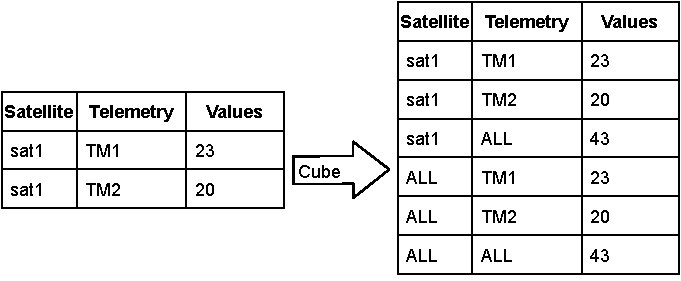
\includegraphics{Figuras/CubeExample.pdf}}
  \end{center}
  \vspace{1mm}
  \legenda{}
  \FONTE{Author}
\end{figure}

\subsection{Data Cube Cells}\label{ch:fun:cube:cells}

A data cube is composed of several subcubes, which are all possible levels of aggregation in the specified dimensions.
Subcubes are composed of base cells and aggregated cells, and an aggregated cell is a cell that uses the special value \textit{ALL} (``$*$'') to demonstrate that it is adding values in one or more dimensions.
A base cell does not use the \textit{ALL} notation, being composed of the lowest level of aggregation~\cite{limaSEQUENTIALPARALLELAPPROACHES2009}.
\autoref{fig:hasse} shows all levels of aggregation of a cube composed of dimensions A, B and C, from the most generic (\textit{apex}) to the most specific (base).

\begin{figure}[!htb]
  \caption{\RED{WRONG, apex and base are inverted}}\label{fig:hasse}
  \vspace{2mm}
  \begin{center}
    \resizebox{5cm}{!}{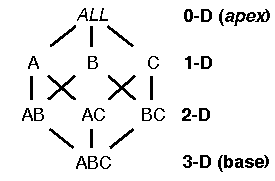
\includegraphics{Figuras/Hasse.pdf}}
  \end{center}
  \vspace{1mm}
  \legenda{A Hasse Diagram of a data cube with three dimensions A, B and C.}
  \FONTE{Author}
\end{figure}

Formally, assuming a $n$-dimensional data cube, a cell $a$ of any subcube is defined by $a = (a_1, a_2, a_3, \ldots, a_n, measures)$.
The cell is $m$-dimensional (from a subcube with $m$ dimensions), if exactly $m$, with $(m \leq n)$, values between $(a_1, a_2, a_3, \ldots, a_n)$ are not ``$*$''.
If $m = n$, then $a$ is a base cell, otherwise $(m < n)$, it is an aggregate cell.

A descending-ancestral relationship can exist between cells.
In a $n$-dimensional data cube, a cell $a = (a_1, a_2, a_3, \ldots, a_n, measures_a)$ with level $i$ is an ancestor of a cell $b = (b_1, b_2, b_3, \ldots, b_n, measures_b)$ of level $j$, and $b$ is a descendant of $a$, if and only if $i < j$ and $1 \leq m \leq n$, where $a_m = b_m$ whenever $a_m \neq *$.
In particular, a $a$ cell is called the parent of a $b$ cell, and $b$ the child of $a$, if and only if $j = i+1$ and $b$ is a descendant of $a$~\cite{hanDataMiningConcepts2011}.

\subsection{Dimensional Modelling}\label{ch:fun:cube:dimm}

There are three main schemes for the dimensional modeling of a data cube: Star Schema, Snowflake Schema and Fact Constellation.
The star schema is the most used, as it contains a central table called the fact table, where most of the data is located, with a smaller set of tables, called dimension tables, for the other dimensions.
\autoref{fig:starschema} shows an example of a star scheme.

\begin{figure}[!htb]
  \caption{Star schema}\label{fig:starschema}
  \vspace{6mm}
  \begin{center}
    \resizebox{4cm}{!}{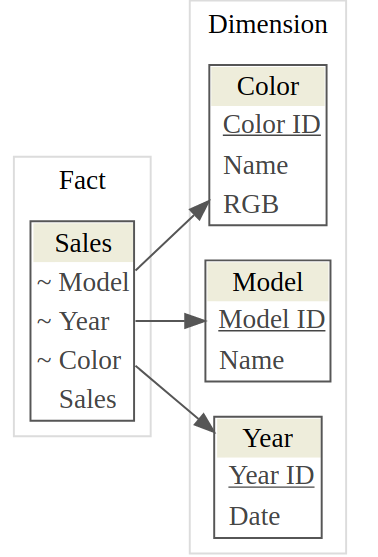
\includegraphics{Figuras/starSchema.png}}
  \end{center}
  \vspace{1mm}
  \legenda{}
  \FONTE{Author}
\end{figure}

The snowflake scheme is a variation of the star scheme, where some dimensions are normalized, dividing the data of the dimension tables into other tables.
This has the advantages of eliminating redundancies in the dimension tables, but it creates problems during the execution of queries since it is necessary to perform join operations with the new tables.
\autoref{fig:snowflakeschema} shows an example of a snowflake scheme.

\begin{figure}[!htb]
  \caption{Snowflake schema}\label{fig:snowflakeschema}
  \vspace{2mm}
  \begin{center}
    \resizebox{6cm}{!}{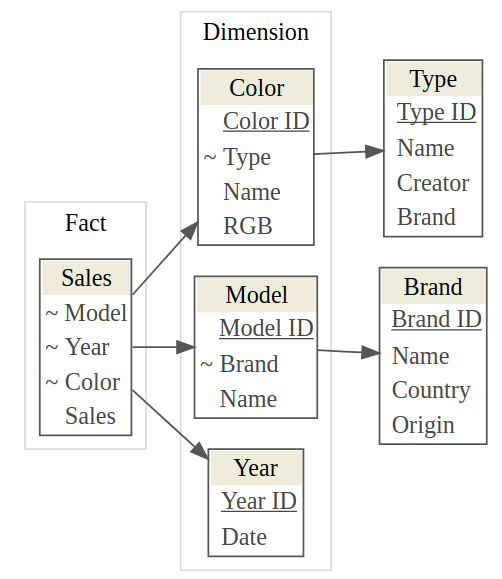
\includegraphics{Figuras/snowflakeSchema.png}}
  \end{center}
  \vspace{1mm}
  \legenda{}
  \FONTE{Author}
\end{figure}

The Fact Constellation uses multiple fact tables, like multiple star schemas but sharing dimension tables, leading to it's name as a group of stars.
\autoref{fig:factconstschema} shows an example of a fact constellation scheme.

\begin{figure}[!htb]
  \caption{Fact Constellatin scheme}\label{fig:factconstschema}
  \vspace{6mm}
  \begin{center}
    \resizebox{6cm}{!}{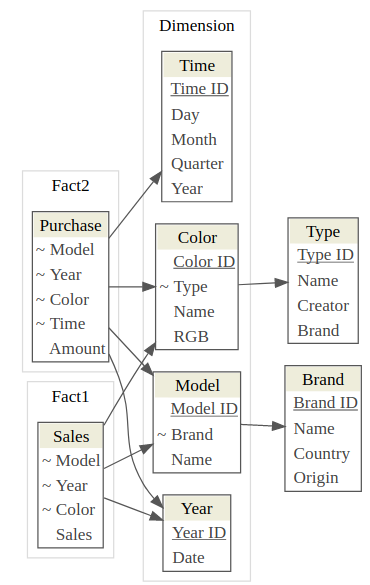
\includegraphics{Figuras/factConstellationSchema.png}}
  \end{center}
  \vspace{2mm}
  \legenda{}
  \FONTE{Author}
\end{figure}

\subsection{Concept Hierarchies}\label{ch:fun:cube:concept}

A concept hierarchy is used to define a mapping sequence between a set of low-level concepts and a set of high-level, more general concepts.
It is a style of grouping and discretization, because it groups the values in order to reduce the cardinality of a dimension~\cite{hanDataMiningConcepts2011}.
They help make the analysis easier to understand, as the operations translate the low-level data into a representation that is easier for the end user, thus facilitating the execution of queries and their subsequent use.

\subsection{Measures}\label{ch:fun:cube:measures}

Each cell of a cube is defined as a pair $\langle (d_1, d_2, \ldots, d_n), measures \rangle$, where $(d_1, d_2, \ldots, d_n)$ represent the possible combinations of attribute values over dimensions.
A measure is calculated for a certain cell by aggregating the data corresponding to the combination of dimensions and values~\cite{hanDataMiningConcepts2011}.
Measurements can be classified into three types: distributive, algebraic and holistic.

A distributive measure is a measure whose calculation can be partitioned and then combined, and the result would be the same if the calculation was performed on the entire data set.
For example, the sum function is distributive: dividing the $N$ data into $n$ sets, and making the sum of each $n$ set, will have the same result as if it were done directly over $N$.

An algebraic measure is a measure that can be calculated with two or more distributive measures.
For example, a measure of average can be calculated by dividing the measure sum by the measure count, which are both distributive.

A measure is holistic if there is no algebraic measure with $M$ arguments that performs the computation.
This means that computing cannot be partitioned, with exact values obtained only if the measure is applied to all data.
Some examples are the measures of mode, standard deviation and median~\cite{hanDataMiningConcepts2011}.

\subsection{OLAP Operations}\label{ch:fun:cube:olapops}

To perform queries in the Data Warehouse, it is necessary to use some operations on the data cube to obtain the appropriate results.
These queries must also be able to go through the hierarchy of concepts of each dimension, as well as follow the dimensional model of the cube, in order to offer a user-friendly interface for interactive analysis~\cite{hanDataMiningConcepts2011}.
Some operations are exemplified in \autoref{fig:olap}, but they usually are:

\begin{itemize}
  \item \textit{Roll-up}: performs aggregation in the data cube, either by navigating the concept hierarchy from a specific level concepts to a more generic one, or by reducing a dimension.
  \item \textit{Drill-down}: the inverse of the roll-up operation, navigates in the hierarchy of concepts from the most generic level to the most specific level, or adds dimensions to the current cube.
  \item \textit{Slice}: performs a selection in a cube dimension, resulting in a subcube focused on that dimension.
  \item \textit{Dice}: defines a subcube by making a selection (slice) in two or more dimensions.
  \item \textit{Pivot}: also called rotation, it allows changing the position of the dimensions in view, changing rows to columns and vice versa.
\end{itemize}

\begin{figure}[!htb]
  \caption{OLAP operations in a Data Cube}\label{fig:olap}
  \vspace{4mm}
  \begin{center}
    \resizebox{15cm}{!}{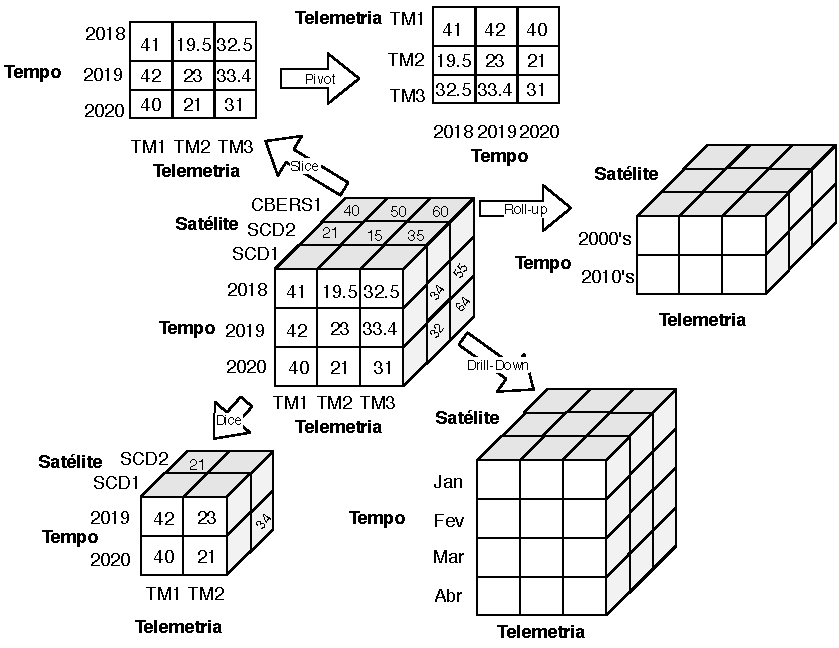
\includegraphics{Figuras/OLAP.pdf}}
  \end{center}
  \vspace{2mm}
  \legenda{\RED{TRANSLATE}}
  \FONTE{Author}
\end{figure}

Depending on the OLAP system, it is possible to execute other operations, like drill-across between multiple fact tables, and drill-through where queries are executed directly on the low-level representation of the data~\cite{hanDataMiningConcepts2011}.

\subsection{Data Cube Computation}\label{ch:fun:cube:comp}

Data cube computation is an essential task, as pre-computing all or part of a data cube can significantly increase DW performance.
However, this task has exponential complexity in relation to the number of dimensions, being called materialization, with complete materialization requiring a large number of cells, and therefore a high memory consumption and time~\cite{hanDataMiningConcepts2011}.

The original calculation of the data cube computation was proposed by~\cite{grayDataCubeRelational1996}, being: given an input relation $R$ with tuples of size $n$, the number of subcubes that can be generated is $2^n$, where $n$ is the number of dimensions of the cube.
For example, assuming a cube with three dimensions \textit{Satellite, Telemetry, Value}, we have $2^3 = 8$ possible subcubes: $\{(satellite, telemetry, value), (satellite, value), (satellite, telemetry),$ $(telemetry, value), (telemetry), (value), (satellite), \emptyset \}$, with $\emptyset$ denoting the empty grouping (base cell, dimensions are not grouped).
% Weird latex thing here...

However, in practice, dimensions can have associated concept hierarchies, as for the time dimension: ``day<month<quarter<semester<year'.
For a cube with $n$ dimensions with multiple concept hierarchies, the total number of subcubes is shown in \autoref{eq:conceptcuboids}.

\begin{equation}
  subcubes = \prod_{i=1}^n (L_i + 1)
\label{eq:conceptcuboids}
\end{equation}

Where $L_i$ is the number of concept levels of the $i$ dimension.
It is necessary to add one to the equation~\ref{eq:conceptcuboids} to denote the virtual level \textit{ALL}.
The size of each subcube also depends on the cardinality of each dimension, that is, the number of distinct values.
While the number of dimensions, concept hierarchies, and cardinality of the cube increases, they also increase the space requirements exponentially, being known as the \textbf{Curse of Dimensionality} in cube computing.

To be able to answer the queries properly, it is necessary to choose a method for subcube computing: non-materialisation, complete materialisation and partial materialisation.

In non-materialisation, the aggregated subcubes are not pre-computed, so the aggregations are computed in query time, which can be extremely slow, but has the lowest memory consumption.

Complete materialization computes all possible aggregations of the cube, generating a complete data cube.
This method generates the best response times, because the aggregations have already been computed, but it requires a large amount of memory.

Partial materialization only computes a selected subset of subcubes, and there are several different techniques for selecting the subcubes to be computed.
One of them is to compute all the subcubes that contain only cells that satisfy a given criterion, specified by the user.
These cubes are called iceberg~\cite{beyerBottomupComputationSparse1999}.

Another technique is to compute small cubes, usually between 3 and 5 dimensions, to form complete cubes.
To answer queries with more dimensions, the combinations between the small subcubes are aggregated.
This technique is called shell fragment, and the cube is called cube shell~\cite{liHighdimensionalOLAPMinimal2004}.

A data cube where cells with identical measurements are encapsulated in a single abstraction, called a closed cell is called a closed cube~\cite{dongxinCCubingEfficientComputation2006}, or quotient cube~\cite{lakshmananQuotientCubeHow2002}.

The choice of partial materialization depends on the required balance between response time and storage space.
However, full cube computation remains relevant, and advances in partial cube computation are generally adopted in full cube computation.
There is also the problem of updating the cube, as each update can cause a partial or complete recomputation of the cube to maintain the correct measurements.

From a base cube, the data cube computation can use the Top-down or Bottom-up strategy for the generation of the remaining subcubes~\cite{hanDataMiningConcepts2011}.

\autoref{fig:topdown} shows the generation of a four-dimensional data cube by the Top-down strategy.
ABCD being a base cube, the three dimension subcubes are: ABC, ABD, ACD and BCD; which can use the results of the base cube to be computed.

\begin{figure}[!hbt]
  \caption{Computing the data cube with the Top-Down strategy}\label{fig:topdown}
  \vspace{4mm}
  \begin{center}
    \resizebox{7cm}{!}{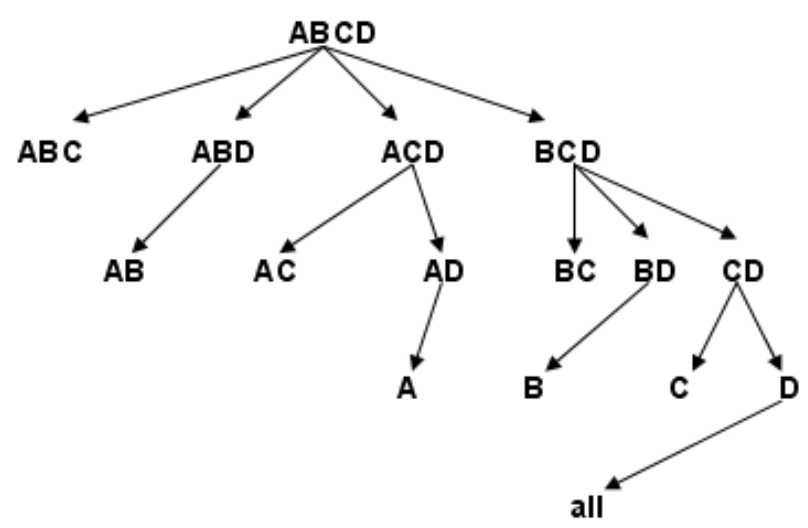
\includegraphics{Figuras/topdown.png}}
  \end{center}
  \vspace{2mm}
  \legenda{}
  \FONTE{~\cite{silva:2015:abordagensParaCubo}.}
\end{figure}

Os resultados da computação do subcubo ACD podem ser utilizados para computar AD, que consequentemente podem ser utilizados para computar A.
Essa computação compartilhada permite que a estratégia \textit{Top-down} compute agregações em múltiplas dimensões.
Os valores agregados intermediários podem ser reutilizados para a computação de subcubos descendentes sucessivos.

A Figura~\ref{fig:bottomup} mostra a geração de um cubo de dados de 4 dimensões por meio da estratégia \textit{Bottom-up}.
Subcubos de poucas dimensões tornam-se pais de subcubos com mais dimensões.
Infelizmente, a computação compartilhada, utilizada na estratégia \textit{Top-down}, não pode ser aplicada quando utilizada a estratégia \textit{Bottom-up}, então cada subcubo descendente necessita ser computado do início.

The results of the ACD subcube computation can be used to compute AD, which consequently can be used to compute A.
This shared computing allows the Top-down strategy to compute aggregations in multiple dimensions.
The intermediate aggregated values can be reused for the computation of successive descending subcubes.

\autoref{fig:bottomup} shows the generation of a 4-dimensional data cube through the Bottom-up strategy.
Low dimensional subcubes become parents of more dimensioned subcubes.
Unfortunately, the shared computing used in the Top-down strategy cannot be applied when using the Bottom-up strategy, so each descending subcube needs to be computed from the beginning.

\begin{figure}[!htb]
  \caption{Computing the data cube with the Bottom-Up strategy}\label{fig:bottomup}
  \vspace{4mm}
  \begin{center}
    \resizebox{8cm}{!}{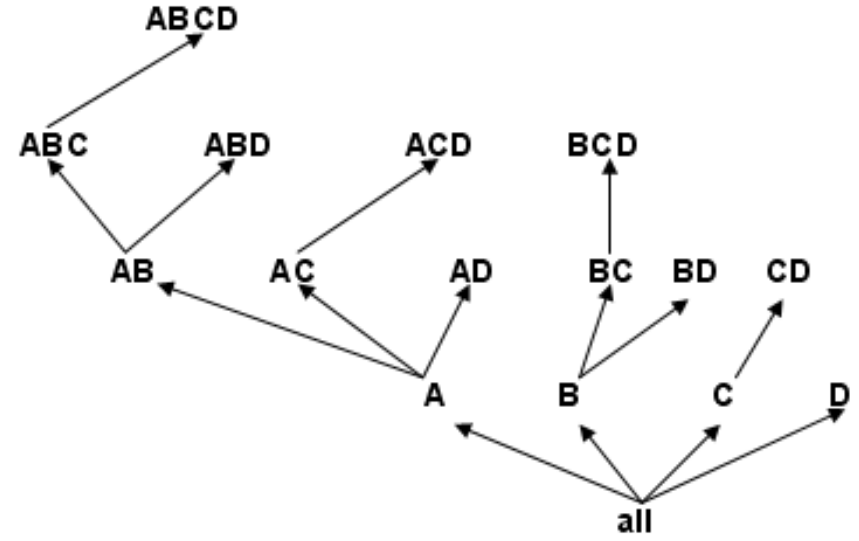
\includegraphics{Figuras/bottomup.png}}
  \end{center}
  \vspace{2mm}
  \legenda{}
  \FONTE{~\cite{silva:2015:abordagensParaCubo}.}
\end{figure}

